	\begin{figure}[H]
		\centering
 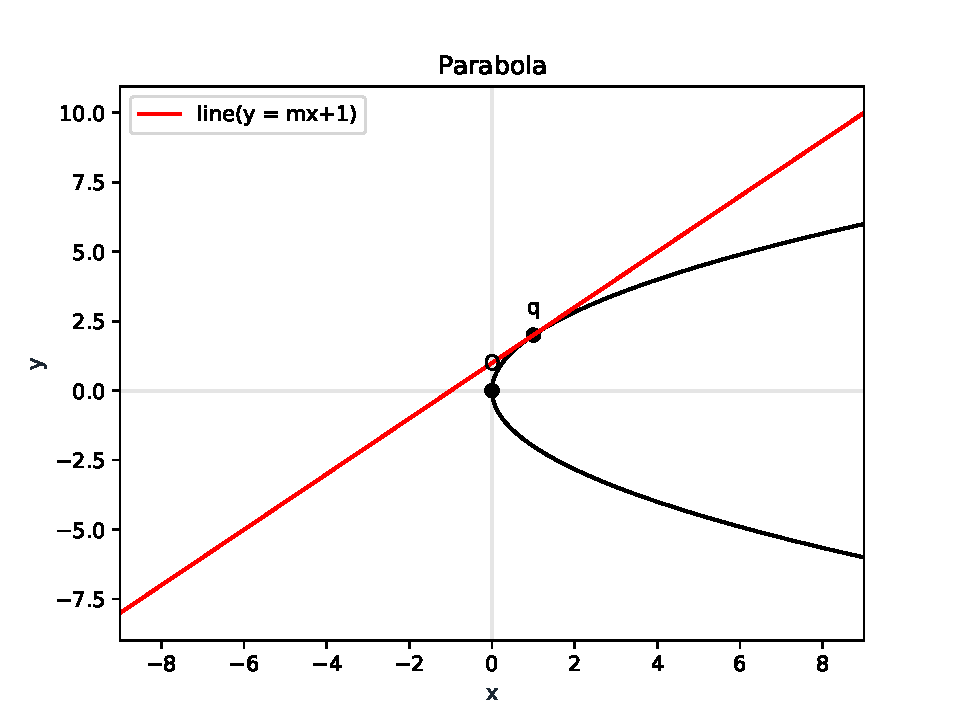
\includegraphics[width=0.75\columnwidth]{chapters/12/6/6/21/figs/im.pdf}
		\caption{}
		\label{fig:12/6/6/21}
  	\end{figure}
The parameters for the given conic are
\begin{align}
    \vec{V} = \myvec{0&0\\0&1}, \vec{u} = \myvec{-2\\0}, f = 0
		\label{eq:12/6/6/21/param}
\end{align}
The given tangent can be expressed in parametric form as
\begin{align}
		\label{eq:12/6/6/21/tangent}
\vec{x} = \vec{e}_2 + \mu\vec{m}
\end{align}
Substituting from 
		\eqref{eq:12/6/6/21/tangent}
		and
		\eqref{eq:12/6/6/21/param}
		in 
	  \eqref{eq:h-tangents-cond}
and solving, we obtain 
\begin{align}
	m = 1.
\end{align}
		See \figref{fig:12/6/6/21}.
